\documentclass[10pt,a4paper]{article}
\usepackage[utf8]{inputenc}
\DeclareUnicodeCharacter{00A0}{~}  % or not it by utf8x
\usepackage[T4]{fontenc}
\usepackage[polish]{babel}
%\usepackage {polski}
\let\lll\undefined
\usepackage{amssymb,amsmath,amsthm}
\usepackage[breaklinks]{hyperref}
\usepackage{graphicx}
\marginparwidth=5.2cm \hoffset=2.5cm \textwidth=12.5cm
\textheight=25.2cm \reversemarginpar \voffset=-1in
%\addtolength{\textheight}{2in}

% Moje pliki latexowe artykułów, które napisałem mają mniej więcej 1100 - 1600 słów
% i to jest trochę ponad 2 strony. A więc celuj w 1000 słów (lub 500 - na 1 stronę), a jak przekroczysz
% to nic się nie stanie. Objętość tekstu nie jest taka ważna, ważniejsza jest treść ;).

\begin{document}
%tytuł
\noindent\textbf{\LARGE Prawdopodobieństwo a informacja}

\medskip
%autor
\noindent\textit{\Large Piotr Migdał}
\marginpar{\footnotesize
    *dr z ICFO--The Institute of Photonic Sciences, Castelldefels (Barcelona), obecnie freelancer z analizy danych \url{http://migdal.wikidot.com}}

\medskip

Filozof może się zadowolić tym, że \emph{``wie, że nic nie wie''}.
Fizyk zaś potrzebuje wiedzieć \emph{ile} nie wie.

Pojęcie \emph{entropii} ma swoje źródło w termodynamice i jest związane z tym jak bardzo nie znamy dokładnego mikrostanu układu (tj. położenia i pędu każdej cząstki).
Tylko gdy wiemy o nim wszystko, możemy w pełni wykorzystać jego energię, przekształcając ją na inne formy.
Gdy nie --- część energii pozostaje niejako uwięziona.

Entropia jest równie cenna w teorii informacji --- pozwala ściśle zmierzyć jak dobrze możemy skompresować daną wiadomość oraz jak bardzo możemy niwelować szum przy jej przesyłaniu.
Przydaje się ona również jako miara losowości i korelacji w różnych narzędziach statystycznych.

O ile entropia jest używana w języku potocznym jako chaos i nieuporządkowanie, to sama wielkość (a konkretniej, \emph{entropia Shannona}) jest ściśle określonym pojęciem:
%
    \marginpar{\footnotesize Częściej jest pisane jako $- \sum_{i=1}^n p_i \log(p_i)$ --- równoważnie ale, moim zdaniem, mniej dydaktycznie.}
%
\begin{align}
    H = \sum_{i=1}^{n} p_i \log \left(\tfrac{1}{p_i} \right),\label{eq:entropia}
\end{align}
%
    \marginpar{\footnotesize Korzystanie z innej podstawy logarytmu, np. $e=2.718\ldots$ przemnoży wynik przez stałą, a zatem odpowiada tylko zmianie jednostek: $\ln(x)=\ln(2)\log_2(x)$. Np. dla podstawy $e$ jednostką jest \emph{nit}.}
%
gdzie $\{p_1, \ldots, p_n\}$ to pewien rozkład prawdopodobieństwa.
Będziemy używać podstawy logarytmu $2$, co odpowiada mierzeniu entropii w \emph{bitach}.
Powyższy wzór ma wiele zastosowań i interpretacji.

Ale zanim przejdziemy do nich, spójrzmy na kilka prostych przykładów.
Gdy nasz rozkład składa się z jednej możliwości, entropia wynosi $1 \log(1) = 0$ bitów --- wszak nie ma tu miejsca na losowość.
Gdy rzucamy uczciwą monetą, entropia to $\tfrac{1}{2} \log(2) + \tfrac{1}{2} \log(2) = 1$ bit.
Entropia jest największa, gdy dla ustalonej liczby zdarzeń wszystkie są równo prawdopodobne --- wtedy wynosi ona $\log(n)$.
Dla kostki do gry z $6$ ścianami to $\log(6)\approx 2.6$.
%
    \marginpar{\footnotesize A jaka jest entropia kolejności talii 52 kart przy tasowaniu?}

Warto pamiętać, że entropia jest zawsze miarą niewiedzy.
Stąd np. kostka na której widzimy wyrzucone dwa oczka ma entropię zero.
Dowiadujemy się dokładnie tyle, o ile entropia zmalała, tu:
%
\begin{align}
    H(\tfrac{1}{6}, \tfrac{1}{6}, \tfrac{1}{6}, \tfrac{1}{6}, \tfrac{1}{6}, \tfrac{1}{6})
    - H(0, 1, 0, 0, 0, 0) = \log(6) - \log(1)
    \approx 2.6.
\end{align}
%
Gdyby ktoś nam powiedział ``wypadło jedno, dwa lub trzy oczka'', nasz wiedza końcowa byłaby niepełna i dowiedzielibyśmy się $\log(6) - \log(3) = 1 $ bit informacji.

    % \marginpar{\footnotesize Z matematycznego punktu widzenia $\lim_{p \to 0} p \log(p) = 0$, z fizycznego --- nie chcemy by dodanie nierealistycznej opcji (tj. z zerowym prawdopodobieństwem) zmieniało wynik.}

Dlaczego potrzebujemy w tym wzorze logarytmu? 
Gdy mamy dwa niezależne zdarzenia, chcemy by ich entropia była sumą entropii składników.
Powiedzmy, że chcemy dowiedzieć się jaki jest znak zodiaku naszego obiektu westchnień oraz czy nas kocha.
Nie powinno grać roli czy dowiemy się na raz jednej informacji czy po kawałku.
Oznaczymy prawdopodobieństwa znaków zodiaku jako $\{p_1, \ldots, p_{12} \}$ oraz uczucie do nas jako $\{q_1, q_2\}$.
Tym samym prawdopodobieństwa poszczególnych, niezależnych zdarzeń to iloczyny: $p_i q_j$.
Zatem jak z entropią?
%
    \marginpar{\footnotesize Czytelnikowi, który zastanawia się czy owe dane są niezależne, polecam zapoznać się z \url{http://bit.ly/dating-zodiac}.}
%

\begin{align}
    \sum_{i=1}^{12} \sum_{j=1}^2 p_i q_j \log(1/(p_i q_j))\label{eq:suma}
    &= \sum_{i=1}^{12} \sum_{j=1}^2 p_i q_j \left( \log(1/p_i) + \log(1/q_j) \right)\\
    &= \sum_{i=1}^{12} \sum_{j=1}^2 p_i q_j \log(1/p_i)
    +\sum_{i=1}^{12} \sum_{j=1}^2 p_i q_j \log(1/q_j)\nonumber\\
    &= \sum_{i=1}^{12} p_i \log(1/p_i)
    + \sum_{j=1}^2 q_j \log(1/q_j),\nonumber
\end{align}
%
zatem entropia niezależnych zdarzeń dodaje się.
W szczególności: $n$ rzutów uczciwą monetą to $n$ bitów entropii.
%
    \marginpar{\footnotesize Wnikliwy czytelnik może sprawdzić, że też $-\log \sum_{i=1}^n p_i^2$ ma tę własność.
    I ogólnie cała rodzina \emph{entropii Rényi'ego}, będących uogólnieniem entropii Shannona;
    przy czym w ogólności nie mają one interpretacji jako informacja.}
%

Na wzór na entropię Shannona można patrzeć również jak na średnią uzyskaną informację.
Zobaczmy to na przykładzie gry w \emph{dwadzieścia pytań}, w której jedna osoba wymyśla jakąś rzecz, a  druga ma za zadanie zgadnąć o co chodzi, zadając po kolei pytania na ``tak'' lub ``nie''.
Można się zastanowić, czy warto zadawać pytania, które są z grubsza \emph{pół na pół} (np. ``Czy to jest żywe?''), czy też takie w których jest niewielka szansa, że dużo się rozjaśni (np. ``Czy to element biżuterii?'').

Powiedzmy, że na starcie jest $m$ możliwych obiektów i każde z nich jest równoprawdopodobne.
Jeśli zadamy pytanie, dla $t$ obiektów odpowiedzią jest ``tak'', dla pozostałych $m-t$ --- ``nie''.
Wiąże się to bezpośrednio z prawdopodobieństwami odpowiedzi:
%
\begin{equation}
    p_{tak} = \tfrac{t}{m}, \qquad p_{nie} = \tfrac{m-t}{m}.
\end{equation}
%
Zatem po uzyskaniu odpowiedzi zbiór możliwych obiektów zmiejsza się do $p_{tak} m$ albo $p_{nie} m$.
Po zadaniu $2$ pytań, dla uposzczenia przyjmując, że z tymi samymi prawdopodobieństwami, dostajemy $4$ możliwości:
$p_{tak} p_{tak} m$, $p_{nie} p_{tak} m$, $p_{tak} p_{nie} m$ albo $p_{nie} p_{nie} m$.
Wygramy w sytuacji, gdy po iluś pytaniach zredukujemy liczbę możliwości do tylko jednej.
O ile może być w tym trochę szczęścia, to przy większej liczbie pytań (a mamy do dyspozycji ich aż $20$), możemy śledzić co się \emph{średnio} stanie.
Skoro przy dodawaniu kolejnych pytań prawdopodobieństwa się mnożą to wielkością, którą chcemy uśredniać jest wspomiany logartym prawdopodobieństwa, czyli otrzymujemy:
%
\begin{equation}
    H = p_{tak} \log \left(\tfrac{1}{p_{tak}} \right) + p_{nie} \log \left(\tfrac{1}{p_{nie}} \right),
\end{equation}
%
--- to samo co \eqref{eq:entropia}.
Po zadaniu $k$ pytań dowiadujemy się średnio $k H$ informacji.
Wielkość ta to $\sum_p p \log(1/p)$, gdzie $p$ to jest prawdopodobieństo uzyskania każdego ciągu odpowiedzi.
Jeśli jej wartość dojdzie do $\log(m)$ to średnio $p = 1/m$, a zatem liczba możliwych obiektów zostanie zredukowana do jednej, czyli: zgadliśmy!
%
    \marginpar{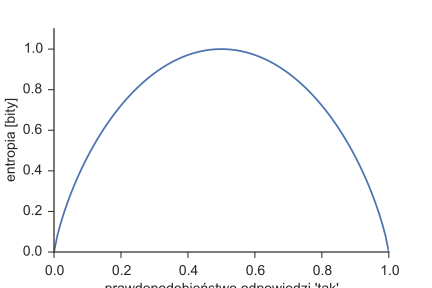
\includegraphics[height=3.5cm]{entropia2}\\
    \footnotesize Entropia przy dwóch możliwościach, $H(p, 1 - p)$, czyli np. rzutu nieuczciwą monetą ($p$ to prawdopodobieństwo orła) lub odpowiedzi na pytanie ($p$ to prawdopodobieństwo ``tak''). Maksimum, równe 1 bitowi, osiąga dla $p=1/2$.}
%
Gdy zadamy pytanie \emph{pół na pół}, to niezależnie od odpowiedzi dowiadujemy się $\log(1/2)=1$ bit informacji.
A co gdy, powiedzmy, zadamy pytanie na które jest tylko $1/1000$ prawdopodobieństwo na ``tak''?
Jest niewielka szansa, że dowiemy się bardzo dużo ($\log(1000)\approx 10$), ale najprawdopodobniej dowiemy się niezbyt wiele.
A sumarycznie, będzie lepiej czy gorzej? Zobaczmy!
%
\begin{equation}
    0.001 \log(\tfrac{1}{0.001}) + 0.999 \log(\tfrac{1}{0.999})\approx 0.0100 + 0.0014 = 0.0114,
\end{equation}
%
czyli bardzo niewiele!
Zresztą, \emph{pół na pół} średnio dostarcza najwięcej informacji --- patrz wykres na marginesie. 

    \marginpar{\footnotesize Pozwolę sobie podkusić Czytelnika do doświadczalnego zmierzenia (na znajomych) entropii pytań oraz entropii pomyślanych obiektów.}

Entropia jest też mocno związana z tym jak dobrze potrafimy skompresować dane.
\emph{Podstawowe twierdzenie Shannona} mówi, że jeśli mamy ciąg $n$ liter,
każda niezależna od innych i z entropią $H$, to nie możemy ich skompresować do długości krótszej niż $n H$.
O ile stoją za tym pewne szczegóły techniczne, główną ideę można oddać zliczając ciągi.
Liczba słów o długości $n$ z alfabetu z $d$ literami to $d^n=2^{n \log(d)}$.
Jeśli chcielibyśmy zakodować owe słowa przy pomocy zer i jedynek
tak, by każde słowo miało swój kod binarnym, potrzebujemy $m = n \log(d)$ bitów.
A co jeśli nie wszystkie litery są równie często używane?
W niektóre ciągi staną się skrajnie mało prawdopodobne gdy przesyłamy wiele liter.

    \marginpar{\includegraphics[height=3.5cm]{litery}\\
    \footnotesize Częstość występowania liter w języku polskim, na podstawie Korpusu IPI PAN.}
%
Dla zwrócenia uwagi, zróbmy to na ciągu z zero i jedynek, z prawdopodobieństwami $p$ i $q$, odpowiednio.
Typowy ciąg o długości $n$ (gdzie $n$ jest duże) będzie miał $n p$ zer i $n q$ jedynek.
Prawdopodobieństwo tego ciągu to $p^{n p}q^{n q}$.
O ile, rzecz jasna, często można otrzymać ciągi z mniejszą lub większą liczbą zer i jedynek

Można pokazać, że nietypowych ciągów (t.j. mających bardzo różną liczbę wystąpień zer i jedynek) jest bardzo mało.
Prawdopodobieństwo musi się sumować do jedności, zatem, skoro typowe ciągi są równoprawdopodobne, liczba ich to:
$p^{-n p}q^{-n q}$.
Czyli, potrzebujemy
%
\begin{align}
    m=n \left( p \log(\tfrac{1}{p}) + q \log(\tfrac{1}{q}) \right)
\end{align}
%
bitów.
Innym słowem, liczba typowych ciągów zer i jedynek rośnie jak $2^{n H}$.
O ile dla niewielkiego $n$ to pewne przybliżenie, to dla $n$ dążącego do nieskończoności zależność jest ścisła.

    \marginpar{\footnotesize  Lektury:\\
    Cosma Schalizi, Information theory\\
    \url{http://bactra.org/notebooks/information-theory.html}\\
    Dissecting the GZIP format\\
    \url{http://www.infinitepartitions.com/art001.html}}
%
Przykładowo, w języku polskim jest używanych $35$ liter (wliczając \texttt{q}, \texttt{x} i \texttt{v} z zapożyczonych słów).
Jednak niektóre litery występują znacznie częściej niż inne np. \texttt{a} stanowi $9\%$ liter, podczas gdy $\texttt{ź}$ --- tylko $0.06\%$.
Entropia rozkładu liter to $4.56$ bitów, czyli dałoby się skompresować polski alfabet do alfabetu z $2^{4.56}\approx 24$ równoprawdopodobnymi literami.
(A pewnie znacznie bardziej, gdyż litery nie występują losowo --- wszakże są połączone w sylaby, słowa, zdania...)  


\end{document}
